\section{Трёхпроходные протоколы}\label{section-three-pass-protocols}
\selectlanguage{russian}

Если между Алисой и Бобом существует канал связи, недоступный для модификации злоумышленником (то есть когда применима модель только пассивного криптоаналитика), то даже без предварительного обмена секретными ключами или другой информацией можно воспользоваться идеями, использованными ранее в криптографии на открытых ключах. После описания RSA в 1978 году, в 1980 Ади Шамир предложил использовать криптосистемы, основанные на коммутативных операциях, для передачи информации без предварительного обмена секретными ключами. Если предположить, что передаваемой информацией является выработанный одной из сторон секретный сеансовый ключ, то в общем виде мы получаем следующий трёхпроходной протокол.

\begin{figure}[!hb]
    \centering
    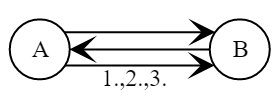
\includegraphics[width=0.5\textwidth]{pic/key_distribution-three-pass}
    \caption{Общая схема взаимодействия участников в трёхпроходных протоколах\label{fig:key_distribution-three-pass}}
\end{figure}

Предварительно:

\begin{itemize}
	\item Алиса и Боб соединены незащищённым каналом связи, открытым для прослушивания (но не для модификации) злоумышленником.
	\item Каждая из сторон имеет пару из открытого и закрытого ключей $K_A$, $k_A$, $K_B$, $k_B$ соответственно.
	\item Сторонами выбрана и используется коммутативная функция шифрования:
	\[\begin{array}{lll}
		D_{A} \left( E_{A} \left( X \right) \right)	= X                                       & \forall X, \left\{ K_A, k_a \right\}; \\
		E_{A} \left( E_{B} \left( X \right) \right)	= E_B \left( E_A \left( X \right) \right) & \forall ~ K_A, K_B, X.
	\end{array}\]
\end{itemize}

Схема взаимодействия участников протокола показана на рис.~\ref{fig:key_distribution-three-pass}. Протокол состоит из трёх проходов с передачей сообщений (отсюда название) и одного заключительного, на котором Боб вычисляет сеансовый ключ.

\begin{protocol}
    \item[(1)] Алиса выбирает новый сеансовый ключ $K$
    \item[{}] $Alice \to \left\{ E_A \left( K \right) \right\} \to Bob$
    \item[(2)] $Bob \to \left\{ E_B \left( E_A \left( K \right) \right) \right\} \to Alice$
    \item[(3)] Алиса, используя коммутативность функции шифрования,
	\[ D_A \left( E_B \left( E_A \left( K \right) \right) \right) = D_A \left( E_A \left( E_B \left( K \right) \right) \right) = E_B \left( K \right). \]
    \item[{}] $Alice \to \left\{ E_B \left( K \right) \right\} \to Bob$
    \item[(4)] Боб расшифровывает $D_B \left( E_B \left( K \right) \right) = K$
\end{protocol}

В результате стороны получают общий секретный ключ $K$.

Общим недостатком всех подобных протоколов является отсутствие аутентификации сторон. Конечно, в случае пассивного криптоаналитика это не требуется, но в реальной жизни всё-таки нужно рассматривать все возможные модели (в том числе активного криптоаналитика) и использовать такие протоколы, которые предполагают взаимную аутентификацию сторон. Также, в отличие от схемы Диффи~---~Хеллмана, новый ключ выбирается инициатором сеанса, что позволяет инициатору, исходя не из лучших побуждений, заставить второго участника использовать устаревший сеансовый ключ.

Если говорить в терминах свойств безопасности, то все представители данного класса протоколов декларируют только аутентификацию ключа (G7). В отличие от схемы Диффи~---~Хеллмана, трёхпроходные протоколы не требуют выбора новых <<мастер>>-ключей для каждого сеанса протокола, из-за чего нельзя гарантировать ни совершенную прямую секретность (G9), ни формирование новых ключей (G10).

\subsection{Тривиальный вариант}

Приведём пример протокола на основе функции XOR (побитовое сложение по модулю 2). Хотя данная функция может использоваться как фундамент для построения систем совершенной криптостойкости (см. главу~\ref{chapter:perfect_secure_systems}), для трёхпроходного протокола это неудачный выбор.

Перед началом протокола обе стороны имеют свои секретные ключи $K_A$ и $K_B$, представляющие собой случайные двоичные последовательности с равномерным распределением символов. Функция шифрования определяется как $E_i( X ) = X \oplus K_i$, где $X$ это сообщение, а $K_i$ -- секретный ключ. Очевидно, что:
\[ \forall i, j, X: E_i \left( E_j \left( X \right) \right) = X \oplus K_j \oplus K_i = X \oplus K_i \oplus K_j = E_j \left( E_i \left( X \right) \right) \]

\begin{protocol}
    \item[(1)] Алиса выбирает новый сеансовый ключ $K$
    \item[{}] $Alice \to \left\{ E_A \left( K \right) = K \oplus K_A \right\} \to Bob$
    \item[(2)] $Bob \to \left\{ E_B \left( E_A \left( K \right) \right) = K \oplus K_A \oplus K_B \right\} \to Alice$
    \item[(3)] Алиса, используя коммутативность функции шифрования,
	\[ D_A \left( E_B \left( E_A \left( K \right) \right) \right) = K \oplus K_A \oplus K_B \oplus K_A = K \oplus K_B = E_B \left( K \right). \]
    \item[{}] $Alice \to \left\{ E_B \left( K \right) = K \oplus K_B \right\} \to Bob$
    \item[(4)] Боб расшифровывает $D_B \left( E_B \left( K \right) \right) = K \oplus K_B \oplus K_B = K$
\end{protocol}

По окончании сеанса протокола Алиса и Боб знают общий сеансовый ключ $K$.

Предложенный выбор коммутативной функции шифрования совершенной секретности является неудачным, так как существуют ситуации, при которых криптоаналитик может определить ключ $K$. Предположим, что криптоаналитик перехватил все три сообщения:
    \[ K \oplus K_A, ~~ K \oplus K_A \oplus K_B, ~~ K \oplus K_B. \]
Сложение по модулю 2 всех трёх сообщений даёт ключ $K$. Поэтому такая система шифрования не применяется.

Теперь приведём протокол надёжной передачи секретного ключа, основанный на экспоненциальной (коммутативной) функции шифрования. Стойкость этого протокола связана с трудностью задачи вычисления дискретного логарифма: при известных значениях $y, g, p$, найти $x$ из уравнения $y = g^x \bmod p$.

\subsection{Бесключевой протокол Шамира}\index{протокол!Шамира бесключевой|(}\label{section-protocols-shamir}

Стороны предварительно договариваются о большом простом числе $p \sim 2^{1024}$. Каждая из сторон выбирает себе по секретному ключу $a$ и $b$. Эти ключи меньше и взаимно просты с $p-1$. Также стороны приготовили по специальному числу $a'$ и $b'$, которые позволяют им расшифровать сообщение, зашифрованное своим ключом:
\[\begin{array}{l}
a' = a{-1} \mod (p-1), \\
a \times a' = 1 \mod (p-1), \\
\forall X: (X^a)^{a'} = X. \\
\end{array}\]

Последнее выражение верно по следствию из малой теоремы Ферма\index{теорема!Ферма малая}. Операции шифрования и расшифрования определяются следующим образом:
\[\begin{array}{lll}
\forall M < p: & C = E( M ) = M^{a}            & \mod p, \\
               & D( C ) = C^{a'}               & \mod p, \\
               & D_A( E_A( M ) ) = M^{aa'} = M & \mod p. \\
\end{array}\]

\begin{protocol}
    \item[(1)] Алиса выбирает новый сеансовый ключ $K < p$
    \item[{}] $Alice \to \left\{ E_A \left( K \right) = K^a \bmod p \right\} \to Bob$
    \item[(2)] $Bob \to \left\{ E_B \left( E_A \left( K \right) \right) = K^{ab} \bmod p \right\} \to Alice$
    \item[(3)] Алиса, используя коммутативность функции шифрования,
	\[ D_A \left( E_B \left( E_A \left( K \right) \right) \right) = K^{aba'} = K^b = E_B \left( K \right) \mod p. \]
    \item[{}] $Alice \to \left\{ E_B \left( K \right) = K^b \right\} \to Bob$
    \item[(4)] Боб расшифровывает $D_B \left( E_B \left( K \right) \right) = K^{bb'} \bmod p = K$
\end{protocol}

По окончании сеанса протокола Алиса и Боб знают общий сеансовый ключ $K$.

Предположим, что криптоаналитик перехватил три сообщения:
\[ \begin{array}{l}
    y_1 = K^a \bmod p, \\
    y_2 = K^{ab} \bmod p, \\
    y_3 = K^b \bmod p. \\
\end{array} \]

Чтобы найти ключ $K$, криптоаналитику надо решить систему из этих трёх уравнений, что имеет очень большую вычислительную сложность, неприемлемую с практической точки зрения, если все три числа $a, b, ab$ достаточно велики. Предположим, что $a$ (или $b$) мало. Тогда, вычисляя последовательные степени $y_3$ (или $y_1$), можно найти $a$ (или $b$), сравнивая результат с $y_2$. Зная $a$, легко найти $a^{-1}\mod(p-1)$ и $K=(y_1)^{a^{-1}}\mod p$.

\index{протокол!Шамира бесключевой|)}

\subsection{Криптосистема Мэсси~---~Омуры}\index{протокол!Мэсси~---~Омуры|(}\index{криптосистема!Мэсси~---~Омуры|(}

В 1982 году Джеймс Мэсси и Джим Омура заявили патент (\langen{James Massey, Jim K. Omura},~\cite{Massey:Omura:1986}), улучшающий (по их мнению) бесключевой протокол Шамира. В качестве операции шифрования вместо возведения в степень в мультипликативной группе $\Z_p^*$ они предложили использовать возведение в степень в поле Галуа $\GF{2^n}$. Секретный ключ каждой стороны (для Алисы -- $a$) должен удовлетворять условиям:
\[ \begin{array}{l}
 a \in \GF{2^n}, \\
 gfd \left( a, x^{ n-1 } + x^{ n-2 } + ... + x + 1 \right) = 1. \\
\end{array} \]

В остальном протокол выглядит аналогично.

\index{протокол!Мэсси~---~Омуры|)}\index{криптосистема!Мэсси~---~Омуры|)}